%%% ДАННЫЙ ФАЙЛ ПРЕДСТАВЛЯЕТ ПРИМЕР ИСПОЛЬЗОВАНИЯ ПАКЕТА pazh2col-win
%%% ДЛЯ ФОРМАТИРОВАНИЯ СТАТЬИ В СТИЛЕ "ПИСЕМ В АСТРОНОМИЧЕСКИЙ ЖУРНАЛ"
%%% С ИСПОЛЬЗОВАНЕМ КОДИРОВКИ WINDOWS-1251.
%%% Автор: Александр Потехин, ФТИ им. А.Ф. Иоффе, 2023 <palex@astro.ioffe.ru>.
%%% ПРЕДОСТАВЛЯЕТСЯ ДЛЯ СВОБОДНОГО ИСПОЛЬЗОВАНИЯ: Creative Commons Zero (СС0).
%%% ПОЖАЛУЙСТА, СООБЩАЙТЕ ОБ ОБНАРУЖЕННЫХ ОШИБКАХ И ПРОБЛЕМАХ ПО ВЫШЕУКАЗАННОМУ АДРЕСУ!

\documentclass{pazh2col-win}

%%% Далее можно подгрузить дополнительные пакеты.
%%% Например, пакет graphicx используется для вставки в текст рисунков:
\usepackage{graphicx}

\begin{document}

%%% Список авторов задается командой \authors.
%%% В квадратных скобках размещается краткий список для верхнего колонтитула на четных страницах:
%%% ФАМИЛИЯ (заглавными буквами) - если автор только один;
%%% ФАМИЛИЯ1, ФАМИЛИЯ2 - если авторов двое;
%%% ФАМИЛИЯ1 и др. - если число авторов больше двух.
%%% В фигурных скобках размещается полный список авторов,
%%% причем каждый следующий добавляется командой \nextauth, имеющей два обязательных аргумента:
%%% в первых фигурных скобках указываются инициалы и фамилия, а во вторых - номера, соответствующие аффилиациям.
%%% Дополнительно, для основного соавтора в квадратных скобках перед фигурными указывается электронный адрес.

\authors[ПЕРВЫЙ и др.]{
  \nextauth[first@extra.terra.edu]{А. Б. Первый}{1,2},
  \nextauth{В. Г. Второв}{1,3},
  \nextauth{Д. Е. Третьяк}{2}
}

%%% Полный и краткий заголовки статьи задаются командой \titles.
%%% В квадратных скобках размещается краткий заголовок для верхнего колонтитула на нечетных страницах
%%% (для корректной печати этого колонтитула команда \titles должна располагаться после команды \authors).
%%% В фигурных скобках дается полное название.

\titles[Необычные звезды]{Объяснение необычных
спектров нового класса нейтронных звезд}

%%% Список аффилиаций задается командой \affiliations, внутри которой каждая следующая аффилиация задается командой \nextaffil. 
%%% При этом последовательная нумерация аффилиаций производится автоматически.
%%% Однако, авторы должны сами проконтролировать соответствие этому списку номеров, указанных в командах \nextauth выше.

\affiliations{
\nextaffil{Внеземной университет, Галактинск,  Россия}
\nextaffil{Школа космоса, Галактинск,  Россия}
\nextaffil{Институт марсианской цивилизации, Планетарск,  Россия}
}

%%% Следующая команда задает содержание строк, в которых указываются ключевые даты:
\def\postupila{Поступила в редакцию ??.??.2023~г.
 \\
После доработки ??.??.20??~г.; принята к публикации ??.??.20??~г.}

%%% Следующая команда задает содержание нижнего колонтитула:
\def\journame{ПИСЬМА В АСТРОНОМИЧЕСКИЙ ЖУРНАЛ ~ том ?? ~ \textnumero~?? ~ 20??}

%%% Аннотация задается как аргумент команды \wideabstract. 
%%% В конце аннотации, внутри этой команды, задаются ключевые слова как аргумент команды \keywords.
%%% После них можно вставить "\doi{}", чтобы зарезервировать место для DOI.

\wideabstract{Проанализированы результаты наблюдений необычных нейтронных звезд, недавно
обнаруженных.....
Предложено объяснение наблюдаемых особенностей в спектрах этих звезд и 
зависимости формы спектра от фазы вращения.
Получены ограничения на параметры, характеризующие  \ldots.
На основе проведенного анализа сделаны выводы о процессах в оболочках таких звезд, влияющих на
\ldots. 
\keywords{нейтронные звезды, рентгеновская астрономия.}
% Заготовка для номера DOI (можно вставить, когда он будет известен):
\doi{10.31857/S...}
} 

%=========================================================

\section{Введение}
\label{introduction}

Пример заготовки Введения.
                           
Нейтронные звезды -- самые компактные\footnote{%
%%% Подстрочное примечание можно вставить при помощи стандартной команды \footnote.
Более компактными могут
быть кварковые звезды, гипотеза  о существовании которых
была выдвинута еще до открытия пульсаров (Иваненко и Курдгелаидзе,
1965), но они не были надежно отождествлены в наблюдениях.}
 из когда-либо
наблюдавшихся звезд: при типичной массе $M\sim
(1$\,--\,$2)\, M_\odot$, радиус нейтронной звезды $R\approx10$\,--\,14
км. ..... Наблюдаемые проявления
нейтронных звезд можно использовать для проверки
теоретических моделей вещества в экстремальных состояниях
(Фортов, 2009). .....

Большинство нейтронных звезд обладают сильными
магнитными полями, недостижимыми в земных лабораториях. 
Гнедин и Сюняев (1974) указали, что спектры
таких звезд могут содержать резонансную электронную
циклотронную линию. Ее обнаружение позволяет 
найти магнитную индукцию $B$ из измерения
циклотронной частоты $\omega_\mathrm{c}=|e|B/(m_e c)$, где $m_e$ и $e$
-- масса и заряд электрона. Открытие  циклотронной линии в спектре
рентгеновского пульсара в двойной системе Геркулес X-1
(Трюмпер и др., 1978) послужило блестящим подтверждением этой
идеи.

Недавно были открыты необычные нейтронные звезды...... 
Возможно, они образуют новый класс.....

В данной статье мы рассмотрим 
характерные особенности спектров этих звезд. Будет предложена физическая модель, позволяющая объяснить
их поведение в разных диапазонах энергии в зависимости от фазы вращения.

%%%%%%%%%%%%%%%%%%%%%%%%%%%%%%%%%%%%%%%%%%%%%%%%%%%%%%%%%
\begin{figure}
\centering
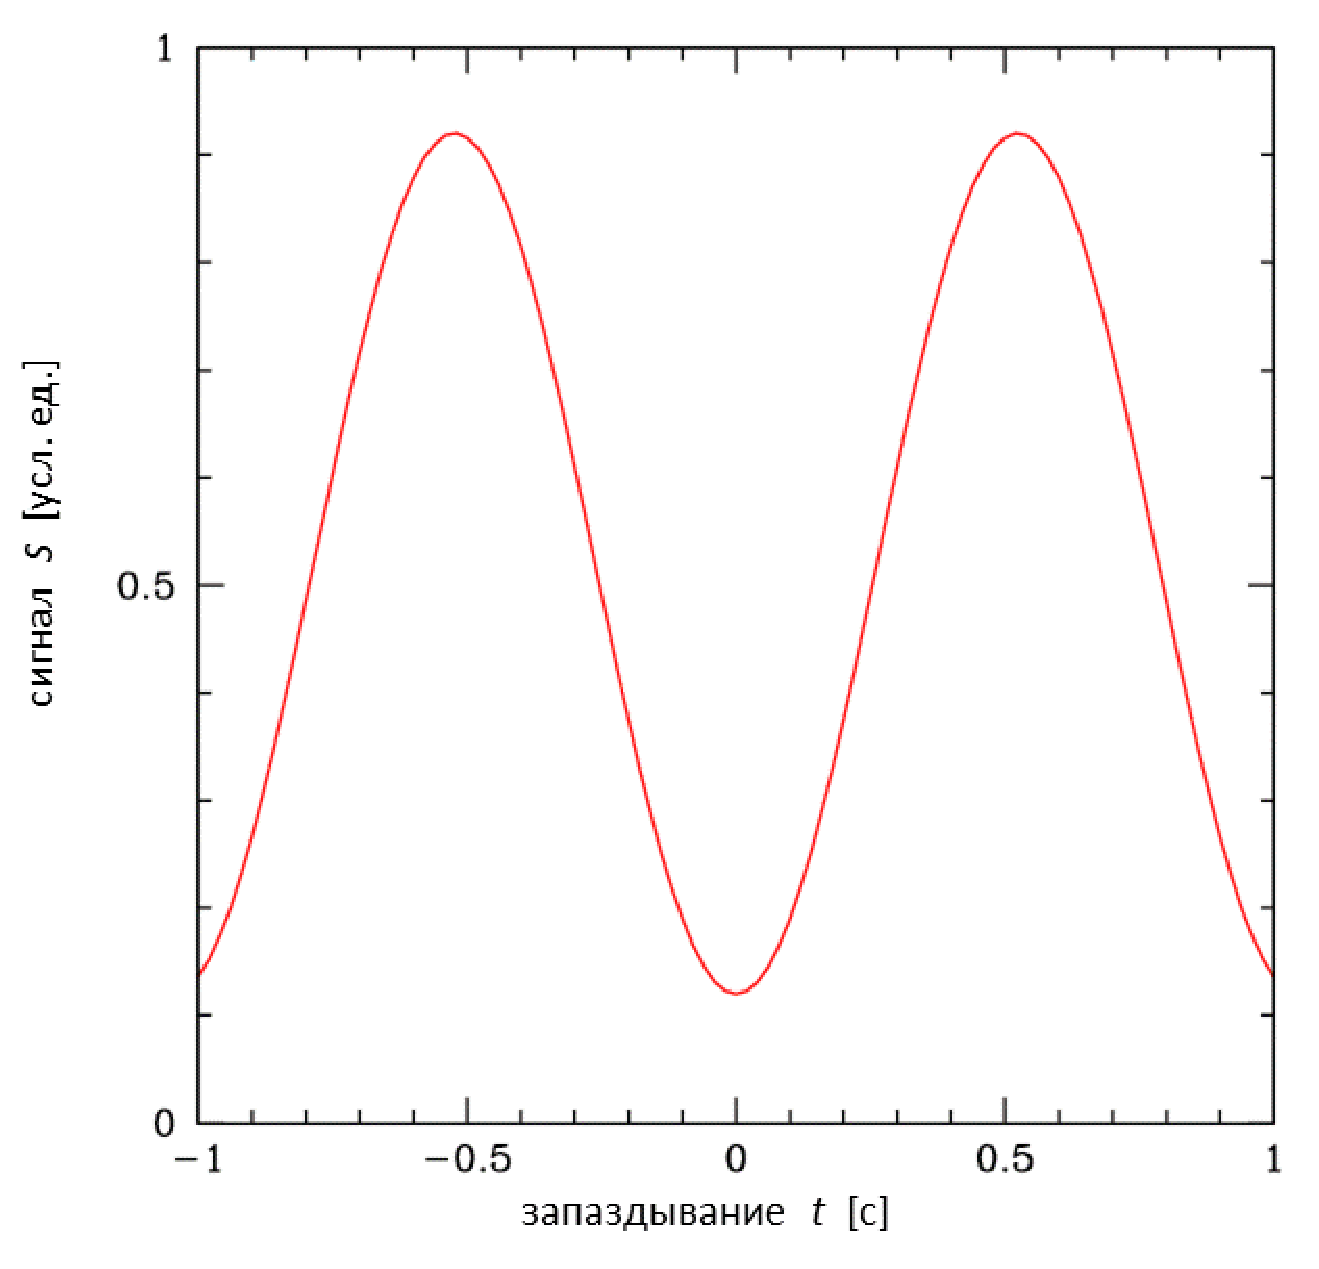
\includegraphics[width=\columnwidth]{fig1exa.eps}
\caption{Пример размещения простого рисунка шириной в одну колонку.}
\label{fig1}
\end{figure}
%%%%%%%%%%%%%%%%%%%%%%%%%%%%%%%%%%%%%%%%%%%%%%%%%%%%%%%%%

%%%%%%%%%%%%%%%%%%%%%%%%%%%%%%%%%%%%%%%%%%%%%%%%%%%%%%%%%
\begin{figure}
\centering
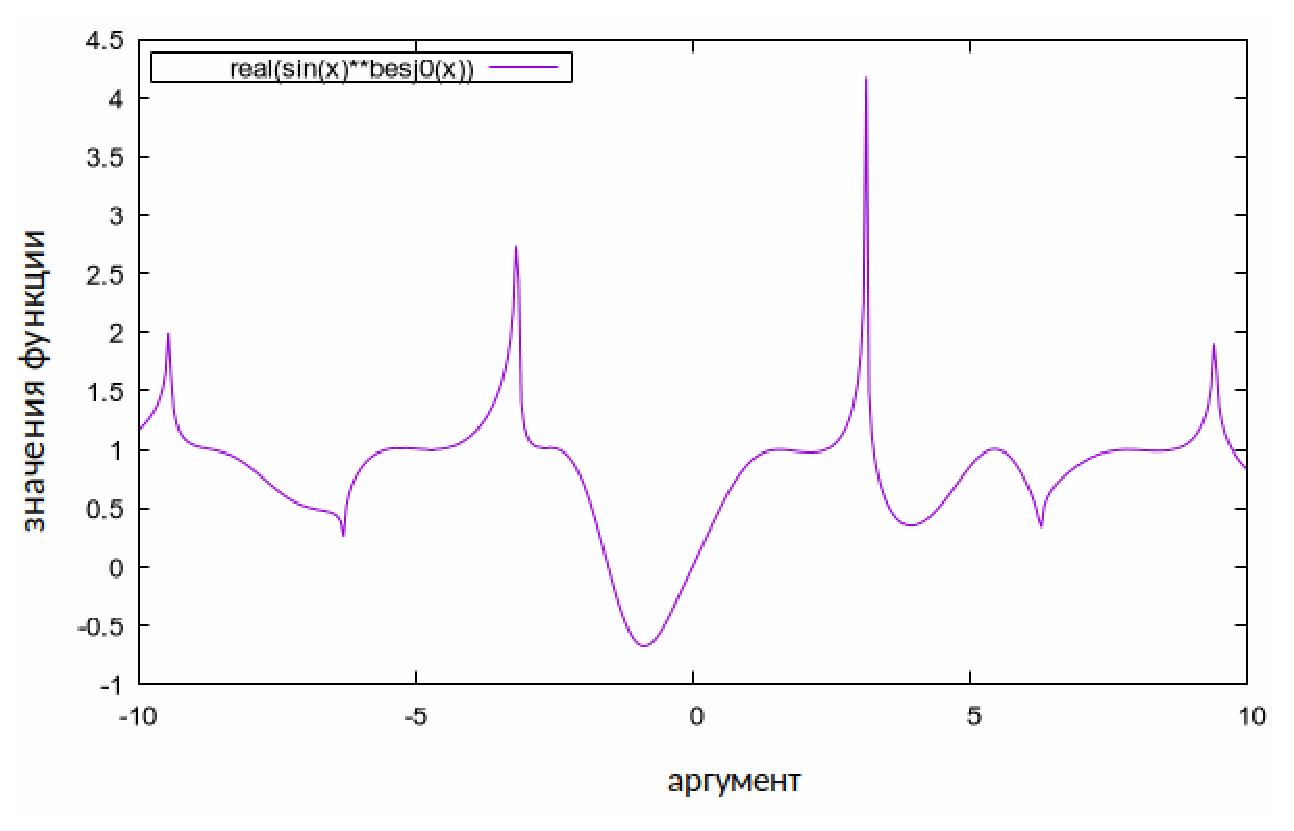
\includegraphics[width=\columnwidth]{fig2exa.eps}
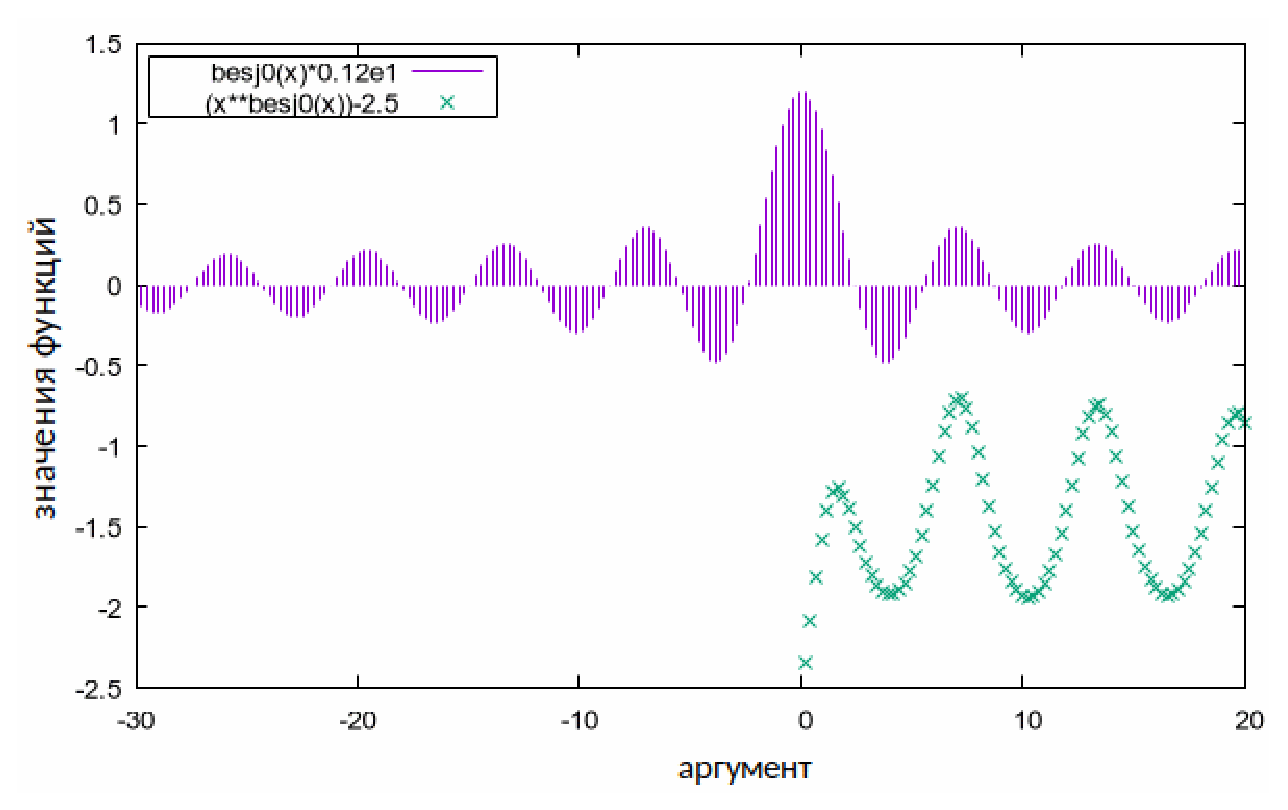
\includegraphics[width=\columnwidth]{fig3exa.eps}
\caption{Пример размещения составного рисунка на ширину колонки.}
\label{fig1a}
\end{figure}
%%%%%%%%%%%%%%%%%%%%%%%%%%%%%%%%%%%%%%%%%%%%%%%%%%%%%%%%%


%%%%%%%%%%%%%%%%%%%%%%%%%%%%%%%%%%%%%%%%%%%%%%%%%%%%%%%%%
\begin{figure*}[t]
\centering
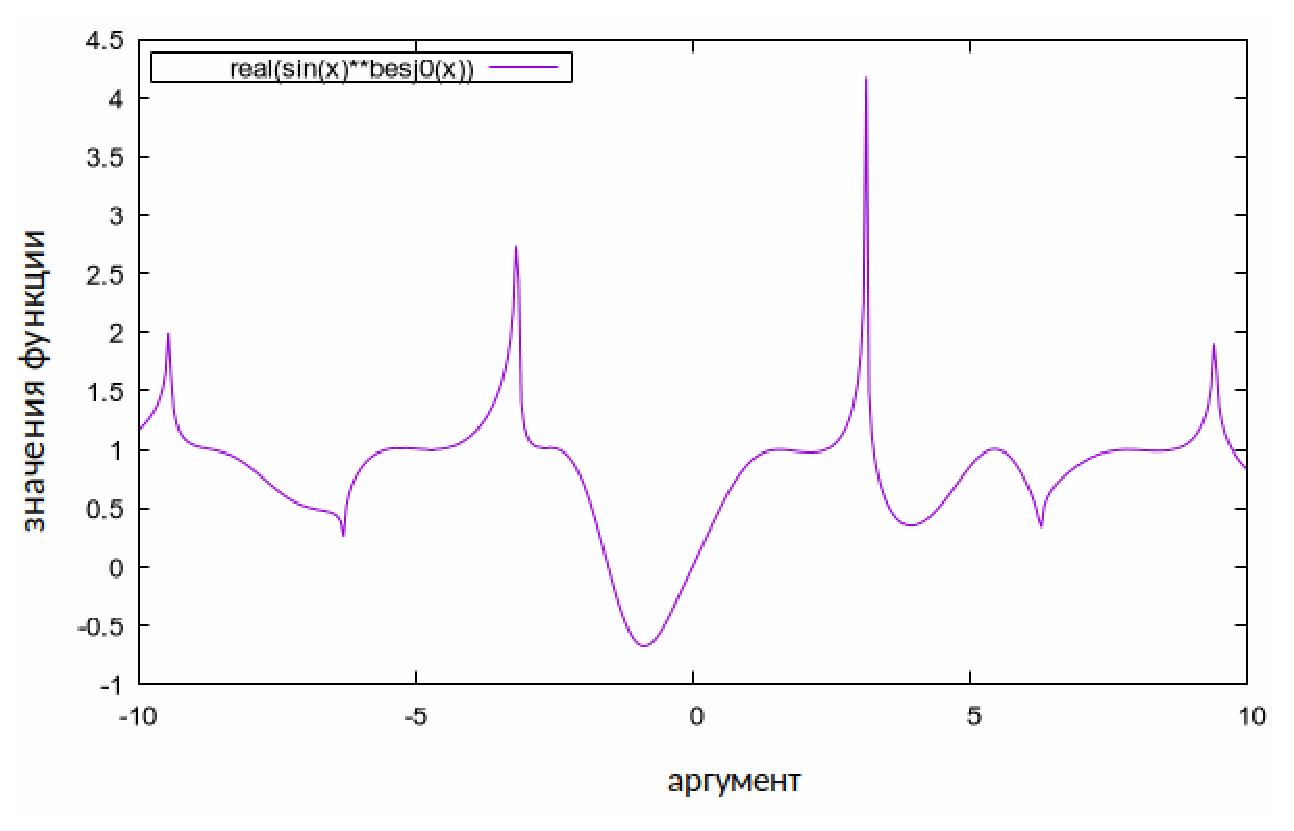
\includegraphics[width=\columnwidth]{fig2exa.eps}
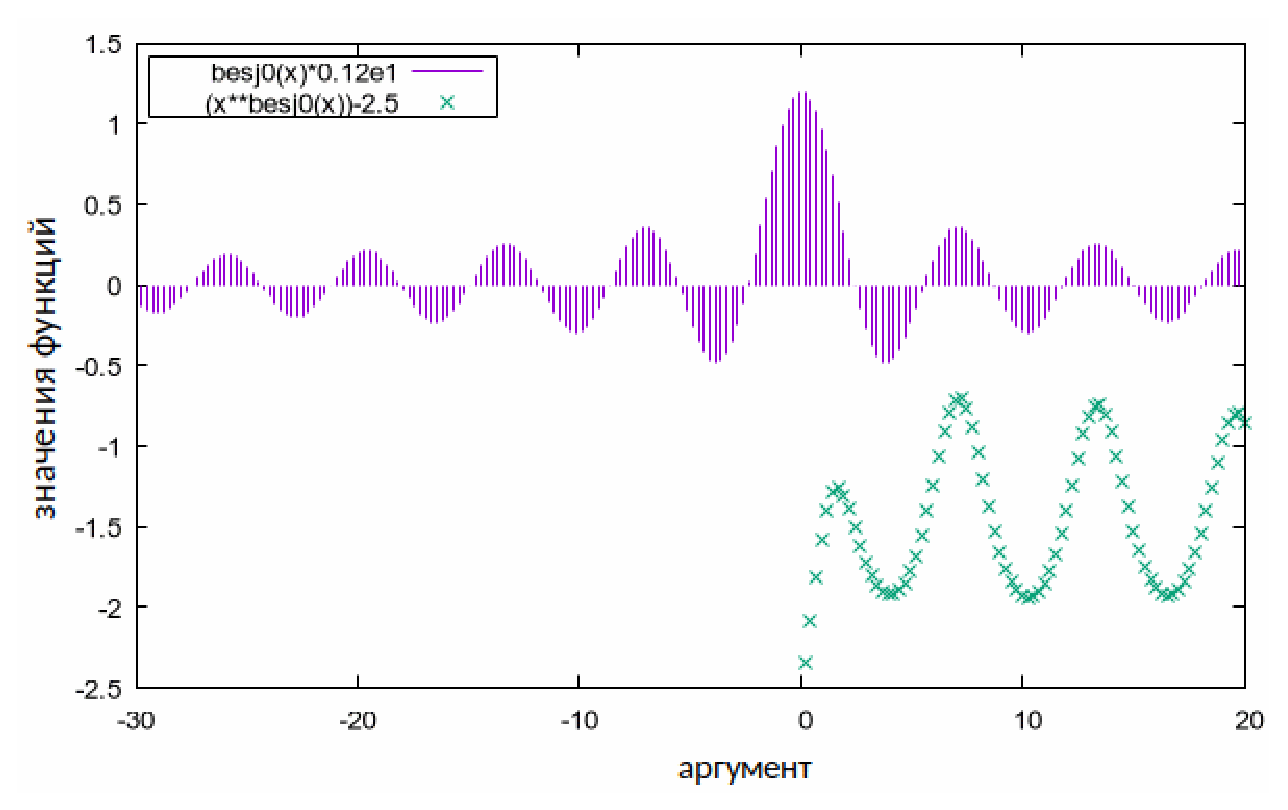
\includegraphics[width=\columnwidth]{fig3exa.eps}
\caption{Пример размещения составного рисунка на всю ширину текста.}
\label{fig2}
\end{figure*}
%%%%%%%%%%%%%%%%%%%%%%%%%%%%%%%%%%%%%%%%%%%%%%%%%%%%%%%%%


%------------------------------------------------------
\section{Основные команды}

В самом начале дается команда
\\
\verb|\documentclass{pazh2col-win}|


Далее можно подгрузить дополнительные пакеты.
Например, для вставки в текст рисунков можно использовать пакет \texttt{graphicx}:
\\
\verb|\usepackage{graphicx}|.

Список авторов задается командой \verb|\authors[]{}|.
В квадратных скобках размещается краткий список для верхнего колонтитула на четных страницах:
ФАМИЛИЯ (заглавными буквами) - если автор только один;
ФАМИЛИЯ1, ФАМИЛИЯ2 - если авторов двое;
ФАМИЛИЯ1 и др. - если число авторов больше двух.
В фигурных скобках размещается полный список авторов,
причем каждый следующий добавляется командой 
\verb|\nextauth[]{}{}|, 
имеющей два обязательных аргумента:
в первых фигурных скобках указываются инициалы и фамилия, а во вторых --
номера, соответствующие аффилиациям данного автора.
Дополнительно, для основного автора в квадратных скобках перед фигурными 
указывается электронный адрес.

 Список аффилиаций задается командой \verb|\affiliations{}|, 
 внутри которой каждая следующая аффилиация задается командой \verb|\nextaffil{}|. 
При этом последовательная нумерация аффилиаций производится автоматически.
Однако, авторы должны сами проконтролировать соответствие этому списку номеров, 
указанных в командах \verb|\nextauth|.

Полный и краткий заголовки статьи задаются командой \verb|\titles[]{}|.
В квадратных скобках размещается краткий заголовок для верхнего колонтитула на нечетных страницах
(для корректной печати этого колонтитула команда \verb|\titles|
 должна располагаться после команды \verb|\authors|).
В фигурных скобках дается полное название.

Следующая команда задает содержание строк, в которых указываются ключевые даты:
\\
\verb|\def\postupila{}|,
\\
-- например:
\\
\verb|\def\postupila{Поступила в редакцию|
\\
\verb|??.??.2023~г. \\ |
\\
\verb|После доработки ??.??.20??~г.;|
\\
\verb| принята к публикации ??.??.20??~г.}|.

Следующая команда задает содержание нижнего колонтитула:
\\
\verb|\def\journame{ПИСЬМА В АСТРОНОМИЧЕСКИЙ|
\\
\verb| ЖУРНАЛ ~ том ?? ~ \textnumero~?? ~ 20??}|.

Аннотация задается как аргумент команды \verb|\wideabstract{}|. 
В конце аннотации, внутри этой команды, задаются ключевые слова 
как аргумент команды \verb|\keywords{}|.
После них можно вставить:
\\
\verb|\doi{}|
\\
-- так мы зарезервируем место для DOI (номер можно указать в фигурных скобках, если он известен).

После этих команд набор основного текста осуществляется, как обычно 
в классе \texttt{article} пакета \LaTeX.

Список литературы предваряется командой \verb|\begin{references}|, 
а завершается командой \verb|\end{references}|.
Библиографическое описание каждой ссылки должно предваряться командой \verb|\reference|
и должно соответствовать Правилам для авторов Писем в Астрономический журнал.
Список литературы должен быть упорядочен по алфавиту.


%------------------------------------------------------
\section{Рисунки}

Рисунок \ref{fig1} -- пример простого рисунка шириной в одну колонку.

Рисунок \ref{fig1a} -- пример составного рисунка шириной в одну колонку.

Рисунок \ref{fig2} -- пример составного рисунка шириной в две колонки.

%------------------------------------------------------
\section{Таблицы}

Таблица \ref{tab1} -- пример небольшой таблицы.

Таблица \ref{tab2} -- пример широкой таблицы. 
На примере последней колонки продемонстрирован 
способ форматирования с фиксированной шириной колонки
и с переносом строк внутри ячеек.



%---------------------------------------------------------------
%%% ПРИМЕР ТАБЛИЦЫ.
%%% ПРИМЕЧАНИЯ К ТАБЛИЦЕ (ПРИ НАЛИЧИИ) МОЖНО ФОРМАТИРОВАТЬ ТАК, КАК ПОКАЗАНО НА ДАННОМ ПРИМЕРЕ

\begin{table}
\centering
\caption{Пример таблицы шириной в одну колонку с примечаниями,
размещенными под таблицей}
\label{tab1} 
%%% СОКРАЩЕНИЯ ДЛЯ ИНДЕКСОВ ПРИМЕЧАНИЙ В ВИДЕ РУССКИХ БУКВ:
\def\marka{$^{\mbox{\small а}}$}
\def\markb{$^{\mbox{\small б}}$}
\def\markv{$^{\mbox{\small в}}$}
%%%%%%%%%%%%%%%%%%%%
\begin{tabular*}{\columnwidth}{l|c|c|c} 
\hline
{Модель}& $kT,$ & $\alpha$\marka\ & $kT_{\rm bb},$\markb \\ 
(см.\ текст)        & кэВ&            & кэВ                \\ 
\hline
A   &              &$2.75\pm0.08$&            \\
B   &$ 49.9\pm5.7 $&             &            \\
C   &$ 27.9\pm2.1 $&$2.51\pm0.10$&            \\
D   &$ 28.8\pm1.9 $&             &            \\
E   &$ 36.3\pm3.5 $&             &$1.7\pm0.7$ \\
F   &$ 16.8\pm3.7 $&$2.08\pm0.57$&$1.7$\markv\    \\ 
\hline
\end{tabular*}
\\
\parbox{\columnwidth}{\vspace*{1ex}
\marka\ фотонный индекс\\
\markb\ чернотельная температура для мягкой компоненты излучения)\\
\markv\ зафиксированный параметр} 
\end{table}
%---------------------------------------------------------------

%---------------------------------------------------------------
%%% ПРИМЕР ШИРОКОЙ ТАБЛИЦЫ.
\begin{table*}[ht]
\begin{center}
\caption{Пример таблицы на всю ширину текста}
\label{tab2}
\begin{tabular*}{\textwidth}{l|c|c|c| p{.3\textwidth}}
\hline
Объект & $R$, км
             & $M$, $M_\odot$ 
             & $d$, кпк
             & Примечание
\\
\hline
EXO 0748$-$676 & $13.7^{+1.0}_{-2.7}$
             & $1.8^{+0.4}_{-0.6}$
             & 7.1
             & Расстояние зафиксировано
\\
EXO 0748$-$676 & $11.8^{+0.7}_{-2.2}-15.2^{+1.5}_{-3.0}$
             & $1.5^{+0.5}_{-0.5}-2.1^{+0.4}_{-0.8}$
             & $5.9-8.3$ 
             & Диапазон оценок для разных расстояний
\\
RX~J1856$-$3754 & $12.1^{+1.3}_{-1.6}$
             & $1.48^{+0.16}_{-0.19}$
             & $0.123^{+0.011}_{-0.015}$
             & Расстояние из измерений параллакса
\\
\hline
\end{tabular*}
\end{center}
\end{table*}
%%%%%%%%%%%%%%%%%%%%%%%%%%%%%%%%%%%%%%%%%%%%%%%%%%%%%%%%%%%


% =========================================================
\section{Пример текста}
\label{section_A}

%------------------------------------------------------
\subsection{Заголовок подраздела}

Как мы отмечали в п.~\ref{introduction}, большинство известных нейтронных звезд
сильно замагничены, и в спектрах некоторых из них наблюдаются циклотронные линии.
Когда в спектре нет опознанной циклотронной линии,
приходится прибегать к косвенным оценкам напряженности магнитного поля.
Для одиночных пульсаров наиболее распространена
оценка по формуле
\begin{equation}
B \approx 3.2\times10^{19} \,C\,
 \sqrt{{P}\dot{{P}}}\textrm{~~Гс},
\label{PPdot} 
\end{equation}
где 
${P}$ -- величина периода в секундах, 
$\dot{{P}}$ -- производная периода по времени, а
$C$ -- коэффициент, зависящий от параметров звезды. Для
вращающегося магнитного диполя в вакууме (Дойч 1955)
$C=R_6^{-3}\,(\sin\alpha)^{-1}\,\sqrt{I_{45}}$, где
$R_6\equiv R/(10^6\mbox{~см})$, $I_{45}$ -- момент инерции в
единицах $10^{45}$ г~см$^2$, а $\alpha$ -- угол между
магнитной осью и осью вращения. В этом случае формула
(\ref{PPdot}) дает магнитную индукцию на экваторе. 
Для оценок в формуле
(\ref{PPdot}) обычно полагают $C=1$ (см., например, Манчестер, Тейлор, 1980).

Моделирование
спектра -- сложная задача, включающая решение уравнений
гидростатического равновесия, баланса энергии и переноса
излучения.....

%------------------------------------------------------
\subsection{Заголовок другого подраздела}
\label{section_AA}

То, насколько важны для звезды эффекты общей теории относительности, определяется ее
параметром компактности
\begin{equation}
  x_\mathrm{g}=r_g/R,
\label{x_g}
\end{equation}
где $R$ -- радиус звезды,
\begin{equation}
  r_g=2GM/c^2\approx 2.95\,M/M_\odot \textrm{ км}
\label{r_g}
\end{equation}
-- гравитационный радиус, а $G$ -- гравитационная
постоянная. Параметр компактности типичной нейтронной
звезды составляет от 1/5 до 1/2, то есть не мал (для
сравнения, у Солнца $x_\mathrm{g}=4.24\times10^{-6}$).

%------------------------------------------------------
\subsubsection{Заголовок подраздела третьего уровня.}
\label{section_BBB}
Обратите внгимание, что в концек такого заголовка должна стоять точка,
а следующий за ним текст должен идти без пропуска строки (т.е.\ без нового абзаца).

Согласно уравнениям (\ref{x_g}) и (\ref{r_g}) в п.~\ref{section_AA}, 
параметр компактности звезды можно вычислить, зная ее массу и радиус.
Соотношение между ними
определяется решением уравнения гидростатического равновесия.....

%=========================================================
\section{Заключение}
\label{sect:concl}

Мы рассмотрели основные особенности .....  Наблюдения
этих звезд успешно описываются при помощи моделей..... 

Предложен простой метод исследования стадии нейтринного охлаждения
внешней коры, который позволил сформулировать универсальное соотношение
для распределения температуры.....


Работа выполнена при поддержке.... (грант \textnumero\ .....).


%%% Список литературы предваряется командой \begin{references}, а завершается командой \end{references}.
%%% Библиографическое описание каждой ссылки должно предваряться командой \reference
%%% и должно соответствовать Правилам для авторов Писем в Астрономический журнал.
%%% Список литературы должен быть упорядочен по алфавиту.
%%% Для сокращенных наименований часто цитируемых журналов можно использовать команды:
%%% \aap - Astron. Astrophys.
%%% \aapr - Astron. Astrophys. Rev.
%%% \aaps - Astron. Astrophys. Suppl. Ser.
%%% \aj - Astron. J.
%%% \ao - Appl. Optics
%%% \apj - Astrophys. J.
%%% \apjl - Astrophys. J.
%%% \apjs - Astrophys. J. Suppl. Ser.
%%% \apss - Astrophys. Space Sci.
%%% \araa - Ann. Rev. Astron. Astrophys.
%%% \asr - Adv. Space Res.
%%% \astl - Astron. Lett.
%%% \atel - Astron. Telegram
%%% \azh - Астрон. журн.
%%% \baas - BAAS       
%%% \iauc - IAU Circ.
%%% \jrasc - JRASC     
%%% \memras - MmRAS
%%% \mnras - Mon. Not. Roy. Astron. Soc.
%%% \nat{%%% \hbox{Nature
%%% \pra - Phys. Rev. A
%%% \prb - Phys. Rev. B
%%% \prc - Phys. Rev. C
%%% \prd - Phys. Rev. D
%%% \prl - Phys. Rev. Lett.    
%%% \pasp - Publ. Astron. Soc. Pacific
%%% \pasj - Publ. Astron. Soc. Japan
%%% \pazh - Письма в Астрон. журн.
%%% \qjras - QJRAS
%%% \skytel - S%%% \&T
%%% \solphys - Solar~Phys.
%%% \sovast - Sov.~Astron.
%%% \sval - Sov.~Astron. Lett.
%%% \ssr - Space~Sci. Rev.
%%% \zap - ZAp

\begin{references}

\reference
Гнедин, Сюняев
(Yu.N. Gnedin and R.A. Sunyaev),
\aap\ \textbf{36}, 379 (1974).

\reference
Дойч (A.J. Deutsch),
Ann.\ d'Astrophys.\ \textbf{18}, 1 (1955).

\reference
Иваненко Д.Д., Курдгелаидзе Д.Ф.,
Астрофизика \textbf{1}, 479 (1965).

\reference
Манчестер Р., Тейлор Дж.,
 \textit{Пульсары} (М.: Мир, 1980).

\reference
Трюмпер и др. (J. Tr\"umper, W. Pietsch, C. Reppin, W. Voges,
R. Staubert, and E. Kendziorra),
\apj\ \textbf{219}, L105 (1978).

\reference
Фортов В.Е.,
УФН \textbf{179}, 653 (2009).

\end{references}

\end{document}
